

\actTitle{Worksheet 4.2A}


\noindent \textbf{Instructions:}  Work together in groups of  3 or 4 to complete the following problems.\\

Student goals:
\begin{itemize}
\item Determine the coordinate of a point on the unit circle given
  either the $x$ or the $y$ value for the coordinate.
\item Given the radian measurement of an angle determine the
  approximate location of the corresponding point on the unit circle
  and determine which quadrant the point is in.
\item Use the definition of trigonometric functions to determine the
  values of the functions given a coordinate on the unit circle.
\item State the domain and range of the trigonometric functions.
\item State the fundamental trigonometric identities.
\item Determine if a basic function is periodic and explain their
  conclusion in terms of the definition of a periodic function.
\item Determine the period of a trigonometric function.
\end{itemize}


\begin{enumerate}

\item Suppose the real number $t$ corresponds to the point
  $P\left(\frac{\sqrt{5}}{5}, \frac{2\sqrt{5}}{5}\right)$ on the unit
  circle.  (The ray at angle $t$ intersects the unit circle at $P$.)
  Evaluate the six trigonometric functions of $t$.
  
  \begin{enumerate} [itemsep=3em]
    \begin{multicols}{2}
    \item $\sin(t)=$ 
    \item $\cos(t)=$ 
    \item $\tan(t)=$ 
      \columnbreak
    \item $\csc(t)=$ 
    \item $\sec(t)=$ 
    \item $\cot(t)=$ 
    \end{multicols}
  \end{enumerate}


\item Use $(x,y)$ coordinates in the unit circle to find the value of
  each trig function at the indicated real number $t=\frac{5\pi}{3}$. 
  \begin{enumerate}[itemsep=3em]
    \begin{multicols}{2}
    \item $\sin\left(\frac{5\pi}{3}\right)=$ 
    \item $\cos\left(\frac{5\pi}{3}\right)=$ 
    \item $\tan\left(\frac{5\pi}{3}\right)=$ 
      \columnbreak
    \item $\csc\left(\frac{5\pi}{3}\right)=$ 
    \item $\sec\left(\frac{5\pi}{3}\right)=$ 
    \item $\cot\left(\frac{5\pi}{3}\right)=$ 
    \end{multicols}
  \end{enumerate}

\clearpage

\item Use $(x,y)$ coordinates in the unit circle to find the value of each trig function at the indicated real number $t=-\frac{5\pi}{4}$.
\begin{enumerate} [itemsep=5em]
\begin{multicols}{2}
\item $\sin\left(-\frac{5\pi}{4}\right)=$ 
\item $\cos\left(-\frac{5\pi}{4}\right)=$ 
\item $\tan\left(-\frac{5\pi}{4}\right)=$ 
\columnbreak
\item $\csc\left(-\frac{5\pi}{4}\right)=$ 
\item $\sec\left(-\frac{5\pi}{4}\right)=$ 
\item $\cot\left(-\frac{5\pi}{4}\right)=$ 
\end{multicols}
\end{enumerate}

\bigskip

\item Evaluate the trig function.
\begin{enumerate}[itemsep=5em]
\begin{multicols}{2}
\item $\sin\left(\frac{3\pi}{4}\right)=$
\item $\tan\left(\frac{4\pi}{3}\right)=$
\item $\sec\left(\frac{5\pi}{6}\right)=$
\columnbreak
\item $\cos\left(\frac{19\pi}{6}\right)=$
\item $\sec\left(-\frac{2\pi}{3}\right)=$
\item $\cot\left(-\frac{\pi}{4}\right)=$ 
\end{multicols}
\end{enumerate}

\bigskip

\item Given $\sin(t)=\frac{3}{7}$ and $\cos(t)=\frac{2\sqrt{10}}{7}$,
  use reciprocal and quotient identities to find the values of the
  other trigonometric functions of $t$.

  \vfill

  \clearpage
  

\item Determine each of the following. (Make a rough sketch of the unit
  circle to help determine the values.)
  \begin{enumerate} 
  \item Use the unit circle to evaluate $\displaystyle \cos\left(\frac{3\pi}{2}\right)$.

  \vfill
  
\item Evaluate $\displaystyle \tan\left(\frac{3\pi}{2}\right)$.

  \vfill
  
\item What trigonometric functions are undefined at
  $\displaystyle t= \frac{3\pi}{2}$?

  \vfill
  
\item Determine all values for $t$ between 0 and $2\pi$ where $\tan(t)$ and $\sec(t)$ are undefined.

  \vfill
  
\end{enumerate}

\item For each trigonometric function, determine all angles between 0
  and $2\pi$ where the function is undefined.

  \begin{enumerate}[itemsep=2em]
    \begin{multicols}{2}
    \item $\sin(t):$
    \item $\csc(t):$
    \item $\tan(t):$
      \columnbreak
    \item $\cos(t):$
    \item $\sec(t):$
    \item $\cot(t):$ 
    \end{multicols}
  \end{enumerate}

\clearpage

\item Use the unit circle to determine the following assuming
  $0\leq t < 2\pi$.
\begin{enumerate}


\item Determine two values of $t$ for which $\csc(t)$ is undefined.
  \vfill

\item Determine two values of $t$ for which $\cos(t)=-\frac{\sqrt{2}}{2}$.
  \vfill

\item Determine two values of $t$ for which $\tan(t)=1$.
  \vfill

\item Determine two values of $t$ for which $\cot(t)=-1$.
  \vfill

\item Determine two values of $t$ for which $\csc(t)=-2$.
  \vfill

\item Determine two values of $t$ for which $\tan(t)=-\sqrt{3}$.
  \vfill

\item Given an angle, $t$, in the first quadrant, at what other angle
  is the cosine the same as $\cos(t)$? 
  In what other quadrants is it guaranteed  the cosine will be different?
  (How does your answer change for the sine?)
  \vfill

\end{enumerate}


\end{enumerate}


\hwTitle{Section 4.2A}

\begin{enumerate}
\item Using the axes below, for each quadrant, determine if the sine
  function is positive or negative. Also indicate whether or not the
  sine is increasing or decreasing for an angle, $t$, in the quadrant.
  
  \begin{tikzpicture}[y=1.5cm, x=1.5cm,font=\sffamily]
    \draw[thin,black,->] (-1.2,0.0) -- (1.2,0.0) node[anchor=south west] {$x$};
    \draw[thin,black,->] (0.0,-1.2) -- (0.0,1.2) node[anchor=south east] {$y$};
  \end{tikzpicture}

\item Using the axes below, for each quadrant, determine if the cosine
  function is positive or negative. Also indicate whether or not the
  sine is increasing or decreasing for an angle, $t$, in the quadrant.
  
  \begin{tikzpicture}[y=1.5cm, x=1.5cm,font=\sffamily]
    \draw[thin,black,->] (-1.2,0.0) -- (1.2,0.0) node[anchor=south west] {$x$};
    \draw[thin,black,->] (0.0,-1.2) -- (0.0,1.2) node[anchor=south east] {$y$};
  \end{tikzpicture}

\item The circle in the diagram below has a radius of 3.  Determine
  the cosine of the angle, $\theta$, given the area, $A$, of the
  shaded sector and use your result to answer the following questions.
  \\ \samepage
  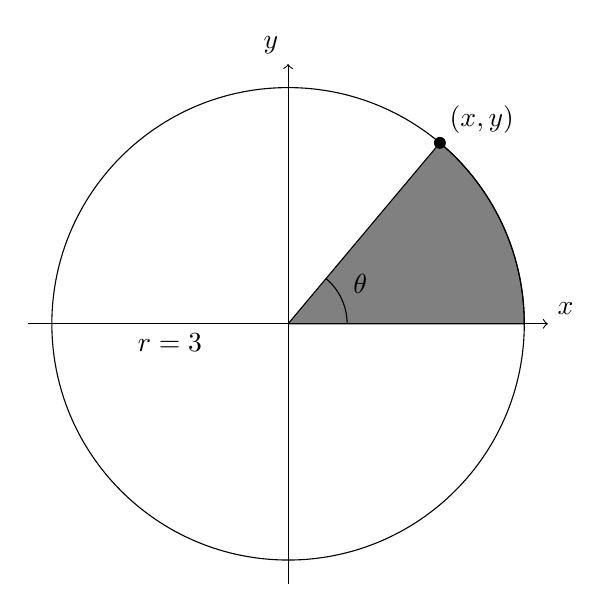
\begin{tikzpicture}[y=1.5cm, x=1.5cm,font=\sffamily]
    \draw[thin,black,fill=gray] (0,0) -- (0:2) arc (0:50:2) -- (0,0);
    \draw[black] (0,0) circle (2);
    \draw[black] (0:0.5) arc (0:50:.5) node[pos=0.4,anchor=south west] {$\theta$};
    \draw[thin,black,->] (-2.2,0.0) -- (2.2,0.0) node[anchor=south west] {$x$};
    \draw[thin,black,->] (0.0,-2.2) -- (0.0,2.2) node[anchor=south east] {$y$};
    \node[black,anchor=north] at (-1,0) {$r=3$};
    \fill[black] (50:2) circle[radius=0.5ex] node[anchor=south west] {$(x,y)$};
    %\node[black,anchor=south east] at (122:2) {$s$};
  \end{tikzpicture}
  
  Determine values of the angle, $\theta$, (between 0 and $2\pi$) where
  each of the following constraints is satisfied:
  \begin{enumerate}
  \item The cosine is positive and increasing.
  \item The cosine is positive and decreasing.
  \item The cosine is negative and increasing.
  \item The cosine is negative and decreasing.
  \end{enumerate}

\item Repeat the previous problem for the sine function.

\item For what values of $t$ between 0 and $2\pi$ is the cosine
  increasing the fastest and where is it decreasing the
  fastest. Briefly explain your reasoning. (Hint: think about a
  small bead moving around the outside at a constant speed.)

\item For what values of $t$ between 0 and $2\pi$ is the sine
  increasing the fastest and where is it decreasing the
  fastest. Briefly explain your reasoning. (Hint: think about a
  small bead moving around the outside at a constant speed.)xs

\end{enumerate}
